\documentclass[9pt,oneside,openany]{memoir}

\iffalse
%font style 1
\usepackage[p,osf]{scholax}
\usepackage{amsmath,amsthm,amssymb}
\usepackage[scaled=1.075,ncf,vvarbb]{newtxmath}
\fi

%font style 2
\usepackage[T1]{fontenc}
\usepackage{amsmath}
\usepackage[fixamsmath]{mathtools}  % Extension to amsmath
\usepackage{amsthm}
\usepackage{amssymb}
\renewcommand*{\mathbf}[1]{\varmathbb{#1}}
\usepackage{newpxtext}
\usepackage{eulerpx}
\usepackage{mathrsfs}
\usepackage{pdfpages}

\usepackage{eucal}
\usepackage{datetime}
    \newdateformat{specialdate}{\THEYEAR\ \monthname\ \THEDAY}
\usepackage[margin=1.5in]{geometry}
\usepackage{fancyhdr}
    \pagestyle{fancy}
    \fancyhf{}
    \cfoot{\scriptsize\thepage}
    \fancyhead[R]{\scalebox{0.8}{\nouppercase{\rightmark}}}
    \fancyhead[L]{\scalebox{0.8}{\nouppercase{\leftmark}}}

    \fancypagestyle{plain}{%
        \fancyhf{}
        \cfoot{\scriptsize\thepage}
        \fancyhead[R]{\scalebox{0.8}{\phantom{a}}}
        \fancyhead[L]{\scalebox{0.8}{Applied Analysis}}
    }
\usepackage{keytheorems}
    \newkeytheoremstyle{def}{
    inherit-style=definition,
    spaceabove=1.5em,
    spacebelow=1.5em,
    postheadspace=0.5em,
    }
    \newkeytheoremstyle{thm}{
    spaceabove=1.5em,
    spacebelow=1.5em,
    postheadspace=0.5em,
    }
    \newkeytheorem{theorem}[
    name = Theorem,
    style=thm,
    numberwithin = section,
    ]
    \newkeytheorem{theorem*}[
    name=Theorem,
    style=thm,
    numbered=false
    ]
    \newkeytheorem{proposition}[
    name = Proposition,
    style=thm,
    numberwithin = section,
    sibling=theorem
    ]
    \newkeytheorem{lemma}[
    name = Lemma,
    style=thm,
    numberwithin = section,
    sibling=theorem
    ]
    \newkeytheorem{corollary}[
    name = Corollary,
    style=thm,
    numberwithin = section,
    sibling=theorem
    ]
    \newkeytheorem{definition}[
    name = Definition,
    style=def,
    numberwithin = section,
    style = definition
    ]
    \newkeytheorem{example}[
    name = Example,
    style=def,
    numberwithin = section,
    style = definition
    ]
    \newkeytheorem{remark}[
    name=Remark,
    style=remark, 
    numbered=false  
    ]
    \newkeytheorem{solution}[
    name=Solution,
    style=remark, 
    numbered=false  
    ]
    \newkeytheorem{question}[
    name=Question,
    style=remark, 
    numbered=false  
    ]
    \newkeytheorem{exercise}[
    name = Exercise,
    style=thm
    ]
    \newkeytheorem{axiom}[name = Axiom]
\usepackage{enumitem}
\usepackage[explicit]{titlesec}
    \titleformat{\chapter}[display]
    {\bfseries\LARGE\raggedright}
    {Chapter {\thechapter}}
    {.1ex minus .1ex}
    {\Large #1}
    \titlespacing{\chapter}
    {3pc}{*3}{40pt}[3pc]

    \titleformat{\section}[block]
    {\normalfont\bfseries\large}
    {}{0pt}
    {\fbox{\strut \S\ \thesection.\ #1}}
    \titlespacing{\section}
    {0pt}{3ex plus .1ex minus .2ex}{3ex plus .1ex minus .2ex}
    \setlength{\fboxsep}{4pt}   % padding inside the box
    \setlength{\fboxrule}{0.6pt} % border thickness
    
    \titleformat{name=\section,numberless}[block]
    {\normalfont\bfseries\large\raggedright}
    {}{0pt}
    {\fbox{\strut #1}}
\usepackage[utf8x]{inputenc}
\usepackage{tikz}
\usepackage{tikz-cd}
\usepackage{float}
\usetikzlibrary{patterns}
\usetikzlibrary{positioning,arrows.meta}
\usetikzlibrary{decorations.pathreplacing}
\usepackage{wasysym}
\usepackage{hyperref}
\usepackage{ulem}
\usepackage{pgfplots}
\usetikzlibrary{patterns}
\usepgfplotslibrary{fillbetween}
\pgfplotsset{compat=1.18}
\usepackage{xcolor}
\usepackage{matlab-prettifier}
\lstdefinestyle{console}{
  basicstyle=\ttfamily\small,
  numbers=none,
  frame=single,
  breaklines=true,
  showstringspaces=false 
}
\definecolor{matlabbg}{HTML}{F2F2F2}
\definecolor{matlabln}{HTML}{6E6E6E}

\lstdefinestyle{editor}{
  style=Matlab-editor,
  backgroundcolor=\color{matlabbg},
  numbers=left,
  numberstyle=\color{matlabln}\ttfamily\scriptsize,
  stepnumber=1,
  numbersep=10pt,
  xleftmargin=2.2em,     % space for line numbers
  frame=single,
  framerule=0pt,         % no border line (keep the box spacing)
  framesep=6pt,
  breaklines=true
}

\renewcommand{\headrulewidth}{0pt} % removes the top/header line
% (optional) if you also want no line above the footer:
\renewcommand{\footrulewidth}{0pt}
%%%%%%%%%%%%%%%%%%%%%%%%%%%%%%%%%%%%%%%%%%%%%%%%%%%%%%%%%%%%%
%%%%%%%%%%%%%%%%%%%%%%%%%%%%%%%%%%%%%%%%%%%%%%%%%%%%%%%%%%%%%
% ============================================================
% makros.tex — reorganized, full restored version
% ============================================================

% ============================================================
% Sha / Cyrillic support notes
% ============================================================

%to make the correct symbol for Sha
%\newcommand\cyr{%
%\renewcommand\rmdefault{wncyr}%
%\renewcommand\sfdefault{wncyss}%
%\renewcommand\encodingdefault{OT2}%
%\normalfont \selectfont} \DeclareTextFontCommand{\textcyr}{\cyr}

% ============================================================
% Math operators
% ============================================================

\DeclareMathOperator{\ab}{ab}
\DeclareMathOperator{\ad}{ad}
\DeclareMathOperator{\adj}{adj}
\DeclareMathOperator{\alg}{alg}
\DeclareMathOperator{\Alt}{Alt}
\DeclareMathOperator{\Ann}{Ann}
\DeclareMathOperator{\arith}{arith}
\DeclareMathOperator{\Aut}{Aut}
\DeclareMathOperator{\Be}{B}
\DeclareMathOperator{\Bd}{Bd}
\DeclareMathOperator{\card}{card}
\DeclareMathOperator{\Char}{char}
\DeclareMathOperator{\csp}{csp}
\DeclareMathOperator{\codim}{codim}
\DeclareMathOperator{\coker}{coker}
\DeclareMathOperator{\coh}{H}
\DeclareMathOperator{\compl}{compl}
\DeclareMathOperator{\conj}{conj}
\DeclareMathOperator{\cont}{cont}
\DeclareMathOperator{\Cov}{Cov}
\DeclareMathOperator{\crys}{crys}
\DeclareMathOperator{\Crys}{Crys}
\DeclareMathOperator{\cusp}{cusp}
\DeclareMathOperator{\diag}{diag}
\DeclareMathOperator{\diam}{diam}
\DeclareMathOperator{\Dom}{Dom}
\DeclareMathOperator{\disc}{disc}
\DeclareMathOperator{\dist}{dist}
\DeclareMathOperator{\Div}{div}
\DeclareMathOperator{\dR}{dR}
\DeclareMathOperator{\Eis}{Eis}
\DeclareMathOperator{\End}{End}
\DeclareMathOperator{\ev}{ev}
\DeclareMathOperator{\eval}{eval}
\DeclareMathOperator{\Eq}{Eq}
\DeclareMathOperator{\Ext}{Ext}
\DeclareMathOperator{\Fil}{Fil}
\DeclareMathOperator{\Fitt}{Fitt}
\DeclareMathOperator{\Frob}{Frob}
\DeclareMathOperator{\G}{G}
\DeclareMathOperator{\Gal}{Gal}
\DeclareMathOperator{\GL}{GL}
\DeclareMathOperator{\Gr}{Gr}
\DeclareMathOperator{\Graph}{Graph}
\DeclareMathOperator{\GSp}{GSp}
\DeclareMathOperator{\GUn}{GU}
\DeclareMathOperator{\Hom}{Hom}
\DeclareMathOperator{\id}{id}
\DeclareMathOperator{\Id}{Id}
\DeclareMathOperator{\Ik}{Ik}
\DeclareMathOperator{\IM}{Im}
\DeclareMathOperator{\Image}{im}
\DeclareMathOperator{\Ind}{Ind}
\DeclareMathOperator{\Inf}{inf}
\DeclareMathOperator{\ins}{ins}
\DeclareMathOperator{\inv}{inv}
\DeclareMathOperator{\Isom}{Isom}
\DeclareMathOperator{\J}{J}
\DeclareMathOperator{\Jac}{Jac}
\DeclareMathOperator{\lcm}{lcm}
\DeclareMathOperator{\length}{length}
\DeclareMathOperator*{\limit}{limit}
\DeclareMathOperator{\Log}{Log}
\DeclareMathOperator{\M}{M}
\DeclareMathOperator{\Mat}{Mat}
\DeclareMathOperator{\N}{N}
\DeclareMathOperator{\Nm}{Nm}
\DeclareMathOperator{\NIk}{N-Ik}
\DeclareMathOperator{\NSK}{N-SK}
\DeclareMathOperator{\new}{new}
\DeclareMathOperator{\obj}{obj}
\DeclareMathOperator{\old}{old}
\DeclareMathOperator{\ord}{ord}
\DeclareMathOperator{\Or}{O}
\DeclareMathOperator{\op}{op}
\DeclareMathOperator{\out}{out}
\DeclareMathOperator{\PGL}{PGL}
\DeclareMathOperator{\PGSp}{PGSp}
\DeclareMathOperator{\rank}{rank}
\DeclareMathOperator{\Ran}{Ran}
\DeclareMathOperator{\rel}{Rel}
\DeclareMathOperator{\Real}{Re}
\DeclareMathOperator{\RES}{res}
\DeclareMathOperator{\Res}{Res}
%\DeclareMathOperator{\Sha}{\textcyr{Sh}}
\DeclareMathOperator{\Sel}{Sel}
\DeclareMathOperator{\semi}{ss}
\DeclareMathOperator{\sgn}{sign}
\DeclareMathOperator{\SK}{SK}
\DeclareMathOperator{\SL}{SL}
\DeclareMathOperator{\SO}{SO}
\DeclareMathOperator{\Sp}{Sp}
\DeclareMathOperator{\Span}{span}
\DeclareMathOperator{\Spec}{Spec}
\DeclareMathOperator{\spin}{spin}
\DeclareMathOperator{\st}{st}
\DeclareMathOperator{\St}{St}
\DeclareMathOperator{\SUn}{SU}
\DeclareMathOperator{\supp}{supp}
\DeclareMathOperator{\Sup}{sup}
\DeclareMathOperator{\Sym}{Sym}
\DeclareMathOperator{\Tam}{Tam}
\DeclareMathOperator{\tors}{tors}
\DeclareMathOperator{\tr}{tr}
\DeclareMathOperator{\Tr}{Tr}
\DeclareMathOperator{\un}{un}
\DeclareMathOperator{\Un}{U}
\DeclareMathOperator{\val}{val}
\DeclareMathOperator{\vol}{vol}

% ============================================================
% General aliases and short macros
% ============================================================

\newcommand{\absgal}{\G_{\bbQ}}
\newcommand{\Loc}{L_{\operatorname{loc}}}
\renewcommand{\k}{\kappa}
\newcommand{\Ff}{F_{f}}
%\newcommand{\ts}{\,^{t}\!}
\newcommand{\lat}{\mathscr{L}}
\newcommand{\ov}[1]{\overline{#1}}
\newcommand{\up}{\upsilon}
\newcommand{\e}{\epsilon}
\newcommand{\tac}{\textasteriskcentered}

%mahesh macros
\newcommand{\tm}{\textrm}

\newcommand{\bone}{\mathbf{1}}
\newcommand{\sign}{\mathrm{sign}}
\newcommand{\eps}{\varepsilon}
\newcommand{\textui}[1]{\underline{\textit{#1}}}

%\newcommand{\ov}{\overline}
%\newcommand{\un}{\underline}
\newcommand{\fin}{\mathrm{fin}}
\newcommand{\nl}{\newline \mbox{}}
\newcommand{\h}[1]{\hspace{#1pt}}
\newcommand{\mtext}[1]{\hspace{6pt}\text{#1}\hspace{6pt}}
\newcommand{\lnorm}{\left\lVert}
\newcommand{\rnorm}{\right\rVert}
\newcommand{\ds}{\displaystyle}
\newcommand{\ts}{\textstyle}
\newcommand{\sfrac}[2]{{}^{#1}\mskip -5mu/\mskip -3mu_{#2}}

% ============================================================
% Category-style operators and contoured variants
% ============================================================

\DeclareMathOperator{\Sets}{S \mkern1.04mu e \mkern1.04mu t \mkern1.04mu s}
    \newcommand{\cSets}{\scalebox{1.02}{\contour{black}{$\Sets$}}}
    
\DeclareMathOperator{\Groups}{G \mkern1.04mu r \mkern1.04mu o \mkern1.04mu u \mkern1.04mu p \mkern1.04mu s}
    \newcommand{\cGroups}{\scalebox{1.02}{\contour{black}{$\Groups$}}}

\DeclareMathOperator{\TTop}{T \mkern1.04mu o \mkern1.04mu p}
    \newcommand{\cTop}{\scalebox{1.02}{\contour{black}{$\TTop$}}}

\DeclareMathOperator{\Htp}{H \mkern1.04mu t \mkern1.04mu p}
    \newcommand{\cHtp}{\scalebox{1.02}{\contour{black}{$\Htp$}}}

\DeclareMathOperator{\Mod}{M \mkern1.04mu o \mkern1.04mu d}
    \newcommand{\cMod}{\scalebox{1.02}{\contour{black}{$\Mod$}}}

\DeclareMathOperator{\Ab}{A \mkern1.04mu b}
    \newcommand{\cAb}{\scalebox{1.02}{\contour{black}{$\Ab$}}}

\DeclareMathOperator{\Rings}{R \mkern1.04mu i \mkern1.04mu n \mkern1.04mu g \mkern1.04mu s}
    \newcommand{\cRings}{\scalebox{1.02}{\contour{black}{$\Rings$}}}

\DeclareMathOperator{\ComRings}{C \mkern1.04mu o \mkern1.04mu m \mkern1.04mu R \mkern1.04mu i \mkern1.04mu n \mkern1.04mu g \mkern1.04mu s}
    \newcommand{\cComRings}{\scalebox{1.05}{\contour{black}{$\ComRings$}}}

\DeclareMathOperator{\hHom}{H \mkern1.04mu o \mkern1.04mu m}
    \newcommand{\cHom}{\scalebox{1.02}{\contour{black}{$\hHom$}}}

% ============================================================
% Mathcal
% ============================================================

\newcommand{\cA}{\mathcal{A}}
\newcommand{\cB}{\mathcal{B}}
\newcommand{\cC}{\mathcal{C}}
\newcommand{\cD}{\mathcal{D}}
\newcommand{\cE}{\mathcal{E}}
\newcommand{\cF}{\mathcal{F}}
\newcommand{\cG}{\mathcal{G}}
\newcommand{\cH}{\mathcal{H}}
\newcommand{\cI}{\mathcal{I}}
\newcommand{\cJ}{\mathcal{J}}
\newcommand{\cK}{\mathcal{K}}
\newcommand{\cL}{\mathcal{L}}
\newcommand{\cM}{\mathcal{M}}
\newcommand{\cN}{\mathcal{N}}
\newcommand{\cO}{\mathcal{O}}
\newcommand{\cP}{\mathcal{P}}
\newcommand{\cQ}{\mathcal{Q}}
\newcommand{\cR}{\mathcal{R}}
\newcommand{\cS}{\mathcal{S}}
\newcommand{\cT}{\mathcal{T}}
\newcommand{\cU}{\mathcal{U}}
\newcommand{\cV}{\mathcal{V}}
\newcommand{\cW}{\mathcal{W}}
\newcommand{\cX}{\mathcal{X}}
\newcommand{\cY}{\mathcal{Y}}
\newcommand{\cZ}{\mathcal{Z}}

% ============================================================
% Mathscrl% 
%============================================================

\newcommand{\scra}{\mathscr{a}}
\newcommand{\scrA}{\mathscr{A}}
\newcommand{\scrb}{\mathscr{b}}
\newcommand{\scrB}{\mathscr{B}}
\newcommand{\scrc}{\mathscr{c}}
\newcommand{\scrC}{\mathscr{C}}
\newcommand{\scrd}{\mathscr{d}}
\newcommand{\scrD}{\mathscr{D}}
\newcommand{\scre}{\mathscr{e}}
\newcommand{\scrE}{\mathscr{E}}
\newcommand{\scrf}{\mathscr{f}}
\newcommand{\scrF}{\mathscr{F}}
\newcommand{\scrg}{\mathscr{g}}
\newcommand{\scrG}{\mathscr{G}}
\newcommand{\scrh}{\mathscr{h}}
\newcommand{\scrH}{\mathscr{H}}
\newcommand{\scri}{\mathscr{i}}
\newcommand{\scrI}{\mathscr{I}}
\newcommand{\scrj}{\mathscr{j}}
\newcommand{\scrJ}{\mathscr{J}}
\newcommand{\scrk}{\mathscr{k}}
\newcommand{\scrK}{\mathscr{K}}
\newcommand{\scrl}{\mathscr{l}}
\newcommand{\scrL}{\mathscr{L}}
\newcommand{\scrm}{\mathscr{m}}
\newcommand{\scrM}{\mathscr{M}}
\newcommand{\scrn}{\mathscr{n}}
\newcommand{\scrN}{\mathscr{N}}
\newcommand{\scro}{\mathscr{o}}
\newcommand{\scrO}{\mathscr{O}}
\newcommand{\scrp}{\mathscr{p}}
\newcommand{\scrP}{\mathscr{P}}
\newcommand{\scrq}{\mathscr{q}}
\newcommand{\scrQ}{\mathscr{Q}}
\newcommand{\scrr}{\mathscr{r}}
\newcommand{\scrR}{\mathscr{R}}
\newcommand{\scrs}{\mathscr{s}}
\newcommand{\scrS}{\mathscr{S}}
\newcommand{\scrt}{\mathscr{t}}
\newcommand{\scrT}{\mathscr{T}}
\newcommand{\scru}{\mathscr{u}}
\newcommand{\scrU}{\mathscr{U}}
\newcommand{\scrv}{\mathscr{v}}
\newcommand{\scrV}{\mathscr{V}}
\newcommand{\scrw}{\mathscr{w}}
\newcommand{\scrW}{\mathscr{W}}
\newcommand{\scrx}{\mathscr{x}}
\newcommand{\scrX}{\mathscr{X}}
\newcommand{\scry}{\mathscr{y}}
\newcommand{\scrY}{\mathscr{Y}}
\newcommand{\scrz}{\mathscr{z}}
\newcommand{\scrZ}{\mathscr{Z}}

% ============================================================
% Mathfrak (missing \fi)
% ============================================================

\newcommand{\fa}{\mathfrak{a}}
\newcommand{\fA}{\mathfrak{A}}
\newcommand{\fb}{\mathfrak{b}}
\newcommand{\fB}{\mathfrak{B}}
\newcommand{\fc}{\mathfrak{c}}
\newcommand{\fC}{\mathfrak{C}}
\newcommand{\fd}{\mathfrak{d}}
\newcommand{\fD}{\mathfrak{D}}
\newcommand{\fe}{\mathfrak{e}}
\newcommand{\fE}{\mathfrak{E}}
\newcommand{\ff}{\mathfrak{f}}
\newcommand{\fF}{\mathfrak{F}}
\newcommand{\fg}{\mathfrak{g}}
\newcommand{\fG}{\mathfrak{G}}
\newcommand{\fh}{\mathfrak{h}}
\newcommand{\fH}{\mathfrak{H}}
\newcommand{\fI}{\mathfrak{I}}
\newcommand{\fj}{\mathfrak{j}}
\newcommand{\fJ}{\mathfrak{J}}
\newcommand{\fk}{\mathfrak{k}}
\newcommand{\fK}{\mathfrak{K}}
\newcommand{\fl}{\mathfrak{l}}
\newcommand{\fL}{\mathfrak{L}}
\newcommand{\fm}{\mathfrak{m}}
\newcommand{\fM}{\mathfrak{M}}
\newcommand{\fn}{\mathfrak{n}}
\newcommand{\fN}{\mathfrak{N}}
\newcommand{\fo}{\mathfrak{o}}
\newcommand{\fO}{\mathfrak{O}}
\newcommand{\fp}{\mathfrak{p}}
\newcommand{\fP}{\mathfrak{P}}
\newcommand{\fq}{\mathfrak{q}}
\newcommand{\fQ}{\mathfrak{Q}}
\newcommand{\fr}{\mathfrak{r}}
\newcommand{\fR}{\mathfrak{R}}
\newcommand{\fs}{\mathfrak{s}}
\newcommand{\fS}{\mathfrak{S}}
\newcommand{\ft}{\mathfrak{t}}
\newcommand{\fT}{\mathfrak{T}}
\newcommand{\fu}{\mathfrak{u}}
\newcommand{\fU}{\mathfrak{U}}
\newcommand{\fv}{\mathfrak{v}}
\newcommand{\fV}{\mathfrak{V}}
\newcommand{\fw}{\mathfrak{w}}
\newcommand{\fW}{\mathfrak{W}}
\newcommand{\fx}{\mathfrak{x}}
\newcommand{\fX}{\mathfrak{X}}
\newcommand{\fy}{\mathfrak{y}}
\newcommand{\fY}{\mathfrak{Y}}
\newcommand{\fz}{\mathfrak{z}}
\newcommand{\fZ}{\mathfrak{Z}}

% ============================================================
% Mathbf
% ============================================================

\newcommand{\bfA}{\mathbf{A}}
\newcommand{\bfB}{\mathbf{B}}
\newcommand{\bfC}{\mathbf{C}}
\newcommand{\bfD}{\mathbf{D}}
\newcommand{\bfE}{\mathbf{E}}
\newcommand{\bfF}{\mathbf{F}}
\newcommand{\bfG}{\mathbf{G}}
\newcommand{\bfH}{\mathbf{H}}
\newcommand{\bfI}{\mathbf{I}}
\newcommand{\bfJ}{\mathbf{J}}
\newcommand{\bfK}{\mathbf{K}}
\newcommand{\bfL}{\mathbf{L}}
\newcommand{\bfM}{\mathbf{M}}
\newcommand{\bfN}{\mathbf{N}}
\newcommand{\bfO}{\mathbf{O}}
\newcommand{\bfP}{\mathbf{P}}
\newcommand{\bfQ}{\mathbf{Q}}
\newcommand{\bfR}{\mathbf{R}}
\newcommand{\bfS}{\mathbf{S}}
\newcommand{\bfT}{\mathbf{T}}
\newcommand{\bfU}{\mathbf{U}}
\newcommand{\bfV}{\mathbf{V}}
\newcommand{\bfW}{\mathbf{W}}
\newcommand{\bfX}{\mathbf{X}}
\newcommand{\bfY}{\mathbf{Y}}
\newcommand{\bfZ}{\mathbf{Z}}

\newcommand{\bfa}{\mathbf{a}}
\newcommand{\bfb}{\mathbf{b}}
\newcommand{\bfc}{\mathbf{c}}
\newcommand{\bfd}{\mathbf{d}}
\newcommand{\bfe}{\mathbf{e}}
\newcommand{\bff}{\mathbf{f}}
\newcommand{\bfg}{\mathbf{g}}
\newcommand{\bfh}{\mathbf{h}}
\newcommand{\bfi}{\mathbf{i}}
\newcommand{\bfj}{\mathbf{j}}
\newcommand{\bfk}{\mathbf{k}}
\newcommand{\bfl}{\mathbf{l}}
\newcommand{\bfm}{\mathbf{m}}
\newcommand{\bfn}{\mathbf{n}}
\newcommand{\bfo}{\mathbf{o}}
\newcommand{\bfp}{\mathbf{p}}
\newcommand{\bfq}{\mathbf{q}}
\newcommand{\bfr}{\mathbf{r}}
\newcommand{\bfs}{\mathbf{s}}
\newcommand{\bft}{\mathbf{t}}
\newcommand{\bfu}{\mathbf{u}}
\newcommand{\bfv}{\mathbf{v}}
\newcommand{\bfw}{\mathbf{w}}
\newcommand{\bfx}{\mathbf{x}}
\newcommand{\bfy}{\mathbf{y}}
\newcommand{\bfz}{\mathbf{z}}

% ============================================================
% Blackboard bold
% ============================================================

\newcommand{\bbA}{\mathbb{A}}
\newcommand{\bbB}{\mathbb{B}}
\newcommand{\bbC}{\mathbb{C}}
\newcommand{\bbD}{\mathbb{D}}
\newcommand{\bbE}{\mathbb{E}}
\newcommand{\bbF}{\mathbb{F}}
\newcommand{\bbG}{\mathbb{G}}
\newcommand{\bbH}{\mathbb{H}}
\newcommand{\bbI}{\mathbb{I}}
\newcommand{\bbJ}{\mathbb{J}}
\newcommand{\bbK}{\mathbb{K}}
\newcommand{\bbL}{\mathbb{L}}
\newcommand{\bbM}{\mathbb{M}}
\newcommand{\bbN}{\mathbb{N}}
\newcommand{\bbO}{\mathbb{O}}
\newcommand{\bbP}{\mathbb{P}}
\newcommand{\bbQ}{\mathbb{Q}}
\newcommand{\bbR}{\mathbb{R}}
\newcommand{\bbS}{\mathbb{S}}
\newcommand{\bbT}{\mathbb{T}}
\newcommand{\bbU}{\mathbb{U}}
\newcommand{\bbV}{\mathbb{V}}
\newcommand{\bbW}{\mathbb{W}}
\newcommand{\bbX}{\mathbb{X}}
\newcommand{\bbY}{\mathbb{Y}}
\newcommand{\bbZ}{\mathbb{Z}}

\newcommand{\Bmu}{\mbox{$\raisebox{-0.59ex}
  {$l$}\hspace{-0.18em}\mu\hspace{-0.88em}\raisebox{-0.98ex}{\scalebox{2}
  {$\color{white}.$}}\hspace{-0.416em}\raisebox{+0.88ex}
  {$\color{white}.$}\hspace{0.46em}$}{}}  %need graphicx and xcolor. this produces blackboard bold mu 

% ============================================================
% Greek-letter aliases
% ============================================================

\newcommand{\jota}{\jmath}

% ============================================================
% Matrices
% ============================================================

\newcommand{\bmat}{\left( \begin{matrix}}
\newcommand{\emat}{\end{matrix} \right)}

\newcommand{\bbmat}{\left[ \begin{matrix}}
\newcommand{\ebmat}{\end{matrix} \right]}

\newcommand{\pmat}{\left( \begin{smallmatrix}}
\newcommand{\epmat}{\end{smallmatrix} \right)}

\newcommand{\mat}[4]{\begin{pmatrix}{#1}&{#2}\\{#3}&{#4}\end{pmatrix}}

% ============================================================
% Residues and averaged integrals
% ============================================================

\newcommand{\res}[1]{\underset{#1}{\RES}\,}

\makeatletter
\newcommand*{\mint}[1]{%
  % #1: overlay symbol
  \mint@l{#1}{}%
}
\newcommand*{\mint@l}[2]{%
  % #1: overlay symbol
  % #2: limits
  \@ifnextchar\limits{%
    \mint@l{#1}%
  }{%
    \@ifnextchar\nolimits{%
      \mint@l{#1}%
    }{%
      \@ifnextchar\displaylimits{%
        \mint@l{#1}%
      }{%
        \mint@s{#2}{#1}%
      }%
    }%
  }%
}
\newcommand*{\mint@s}[2]{%
  % #1: limits
  % #2: overlay symbol
  \@ifnextchar_{%
    \mint@sub{#1}{#2}%
  }{%
    \@ifnextchar^{%
      \mint@sup{#1}{#2}%
    }{%
      \mint@{#1}{#2}{}{}%
    }%
  }%
}
\def\mint@sub#1#2_#3{%
  \@ifnextchar^{%
    \mint@sub@sup{#1}{#2}{#3}%
  }{%
    \mint@{#1}{#2}{#3}{}%
  }%
}
\def\mint@sup#1#2^#3{%
  \@ifnextchar_{%
    \mint@sup@sub{#1}{#2}{#3}%
  }{%
    \mint@{#1}{#2}{}{#3}%
  }%
}
\def\mint@sub@sup#1#2#3^#4{%
  \mint@{#1}{#2}{#3}{#4}%
}
\def\mint@sup@sub#1#2#3_#4{%
  \mint@{#1}{#2}{#4}{#3}%
}
\newcommand*{\mint@}[4]{%
  % #1: \limits, \nolimits, \displaylimits
  % #2: overlay symbol: -, =, ...
  % #3: subscript
  % #4: superscript
  \mathop{}%
  \mkern-\thinmuskip
  \mathchoice{%
    \mint@@{#1}{#2}{#3}{#4}%
        \displaystyle\textstyle\scriptstyle
  }{%
    \mint@@{#1}{#2}{#3}{#4}%
        \textstyle\scriptstyle\scriptstyle
  }{%
    \mint@@{#1}{#2}{#3}{#4}%
        \scriptstyle\scriptscriptstyle\scriptscriptstyle
  }{%
    \mint@@{#1}{#2}{#3}{#4}%
        \scriptscriptstyle\scriptscriptstyle\scriptscriptstyle
  }%
  \mkern-\thinmuskip
  \int#1%
  \ifx\\#3\\\else_{#3}\fi
  \ifx\\#4\\\else^{#4}\fi  
}
\newcommand*{\mint@@}[7]{%
  % #1: limits
  % #2: overlay symbol
  % #3: subscript
  % #4: superscript
  % #5: math style
  % #6: math style for overlay symbol
  % #7: math style for subscript/superscript
  \begingroup
    \sbox0{$#5\int\m@th$}%
    \sbox2{$#5\int_{}\m@th$}%
    \dimen2=\wd0 %
    % => \dimen2 = width of \int
    \let\mint@limits=#1\relax
    \ifx\mint@limits\relax
      \sbox4{$#5\int_{\kern1sp}^{\kern1sp}\m@th$}%
      \ifdim\wd4>\wd2 %
        \let\mint@limits=\nolimits
      \else
        \let\mint@limits=\limits
      \fi
    \fi
    \ifx\mint@limits\displaylimits
      \ifx#5\displaystyle
        \let\mint@limits=\limits
      \fi
    \fi
    \ifx\mint@limits\limits
      \sbox0{$#7#3\m@th$}%
      \sbox2{$#7#4\m@th$}%
      \ifdim\wd0>\dimen2 %
        \dimen2=\wd0 %
      \fi
      \ifdim\wd2>\dimen2 %
        \dimen2=\wd2 %
      \fi
    \fi
    \rlap{%
      $#5%
        \vcenter{%
          \hbox to\dimen2{%
            \hss
            $#6{#2}\m@th$%
            \hss
          }%
        }%
      $%
    }%
  \endgroup
}
\newcommand{\avg}{\mint{-}}
\makeatother

% ============================================================
% Comments and drafting helpers
% ============================================================

%Comments
\newcommand{\com}[1]{\vspace{5 mm}\par \noindent
\marginpar{\textsc{Comment}} \framebox{\begin{minipage}[c]{0.95
\textwidth} \tt #1 \end{minipage}}\vspace{5 mm}\par}

% ============================================================
% Arrows
% ============================================================

\newcommand{\hooktwoheadrightarrow}{%
  \hookrightarrow\mathrel{\mspace{-15mu}}\rightarrow
}

\makeatletter
\newcommand{\xhooktwoheadrightarrow}[2][]{%
  \lhook\joinrel
  \ext@arrow 0359\rightarrowfill@ {#1}{#2}%
  \mathrel{\mspace{-15mu}}\rightarrow
}
\makeatother

\makeatletter
\newcommand*{\da@rightarrow}{\mathchar"0\hexnumber@\symAMSa 4B }
\newcommand*{\da@leftarrow}{\mathchar"0\hexnumber@\symAMSa 4C }
\newcommand*{\xdashrightarrow}[2][]{%
  \mathrel{%
    \mathpalette{\da@xarrow{#1}{#2}{}\da@rightarrow{\,}{}}{}%
  }%
}
\newcommand{\xdashleftarrow}[2][]{%
  \mathrel{%
    \mathpalette{\da@xarrow{#1}{#2}\da@leftarrow{}{}{\,}}{}%
  }%
}
\newcommand*{\da@xarrow}[7]{%
  % #1: below
  % #2: above
  % #3: arrow left
  % #4: arrow right
  % #5: space left 
  % #6: space right
  % #7: math style 
  \sbox0{$\ifx#7\scriptstyle\scriptscriptstyle\else\scriptstyle\fi#5#1#6\m@th$}%
  \sbox2{$\ifx#7\scriptstyle\scriptscriptstyle\else\scriptstyle\fi#5#2#6\m@th$}%
  \sbox4{$#7\dabar@\m@th$}%
  \dimen@=\wd0 %
  \ifdim\wd2 >\dimen@
    \dimen@=\wd2 %   
  \fi
  \count@=2 %
  \def\da@bars{\dabar@\dabar@}%
  \@whiledim\count@\wd4<\dimen@\do{%
    \advance\count@\@ne
    \expandafter\def\expandafter\da@bars\expandafter{%
      \da@bars
      \dabar@ 
    }%
  }%  
  \mathrel{#3}%
  \mathrel{%   
    \mathop{\da@bars}\limits
    \ifx\\#1\\%
    \else
      _{\copy0}%
    \fi
    \ifx\\#2\\%
    \else
      ^{\copy2}%
    \fi
  }%   
  \mathrel{#4}%
}
\makeatother

% ============================================================
% Relation and delimiter spacing
% ============================================================

\renewcommand{\geq}{\geqslant}
\renewcommand{\leq}{\leqslant}
\newcommand{\midd}{\hspace{4pt}\middle|\hspace{4pt}}

% ============================================================
% Left Right Updated Deliminators
% ============================================================

\makeatletter
\NewDocumentCommand\Left{O{}}{%
    \IfValueTF{#1}{\notblank{#1}{\mathopen\bBigg@{#1}}{\left}}{\left}}
\NewDocumentCommand\Right{O{}}{%
    \IfValueTF{#1}{\notblank{#1}{\mathopen\bBigg@{#1}}{\right}}{\right}}
\makeatother

% ============================================================
% Restrictions
% ============================================================

\newcommand{\littletaller}{\mathchoice{\vphantom{\big|}}{}{}{}}
\newcommand\restr[2]{{% we make the whole thing an ordinary symbol
  \left.\kern-\nulldelimiterspace % automatically resize the bar with \right
  #1 % the function
  \littletaller % pretend it's a little taller at normal size
  \right|_{#2} % this is the delimiter
  }}

% ============================================================
% Chapter title formatting
% ============================================================

\newcommand{\chnum}{\titleformat
{\chapter} % command
[display] % shape
{\centering} % format
{\Huge \color{black} \shadowbox{\thechapter}} % label
{-0.5em} % sep (space between the number and title)
{\LARGE \color{black} \underline} % before-code
}

\newcommand{\chunnum}{\titleformat
{\chapter} % command
[display] % shape
{} % format
{} % label
{0em} % sep
{ \begin{flushright} \begin{tabular}{r}  \Huge \color{black}
} % before-code
[
\end{tabular} \end{flushright} \normalsize
] % after-code
}



\begin{document}
\begin{center}
    {\Large Math 502 \\[0.1in]Homework \#5}\\[.175in]
    {Name:} {\underline{Gianluca Crescenzo\hspace*{2in}}}\\[0.15in]
    \end{center}
    \vspace{4pt}
%%%%%%%%%%%%%%%%%%%%%%%%%%%%%%%%%%%%%%%%%%%%%%%%%%
%%%%%%%%%%%%%%%%%%%%%%%%%%%%%%%%%%%%%%%%%%%%%%%%%%
%%%%%%%%%%%%%%%%%%%%%%%%%%%%%%%%%%%%%%%%%%%%%%%%%%
\begin{exercise}[manual-num={8.1}]

\end{exercise}
\begin{solution}
    Below is the stability region for the TR-BDF2 method.
    
    \phantom{a}
    \begin{center}
    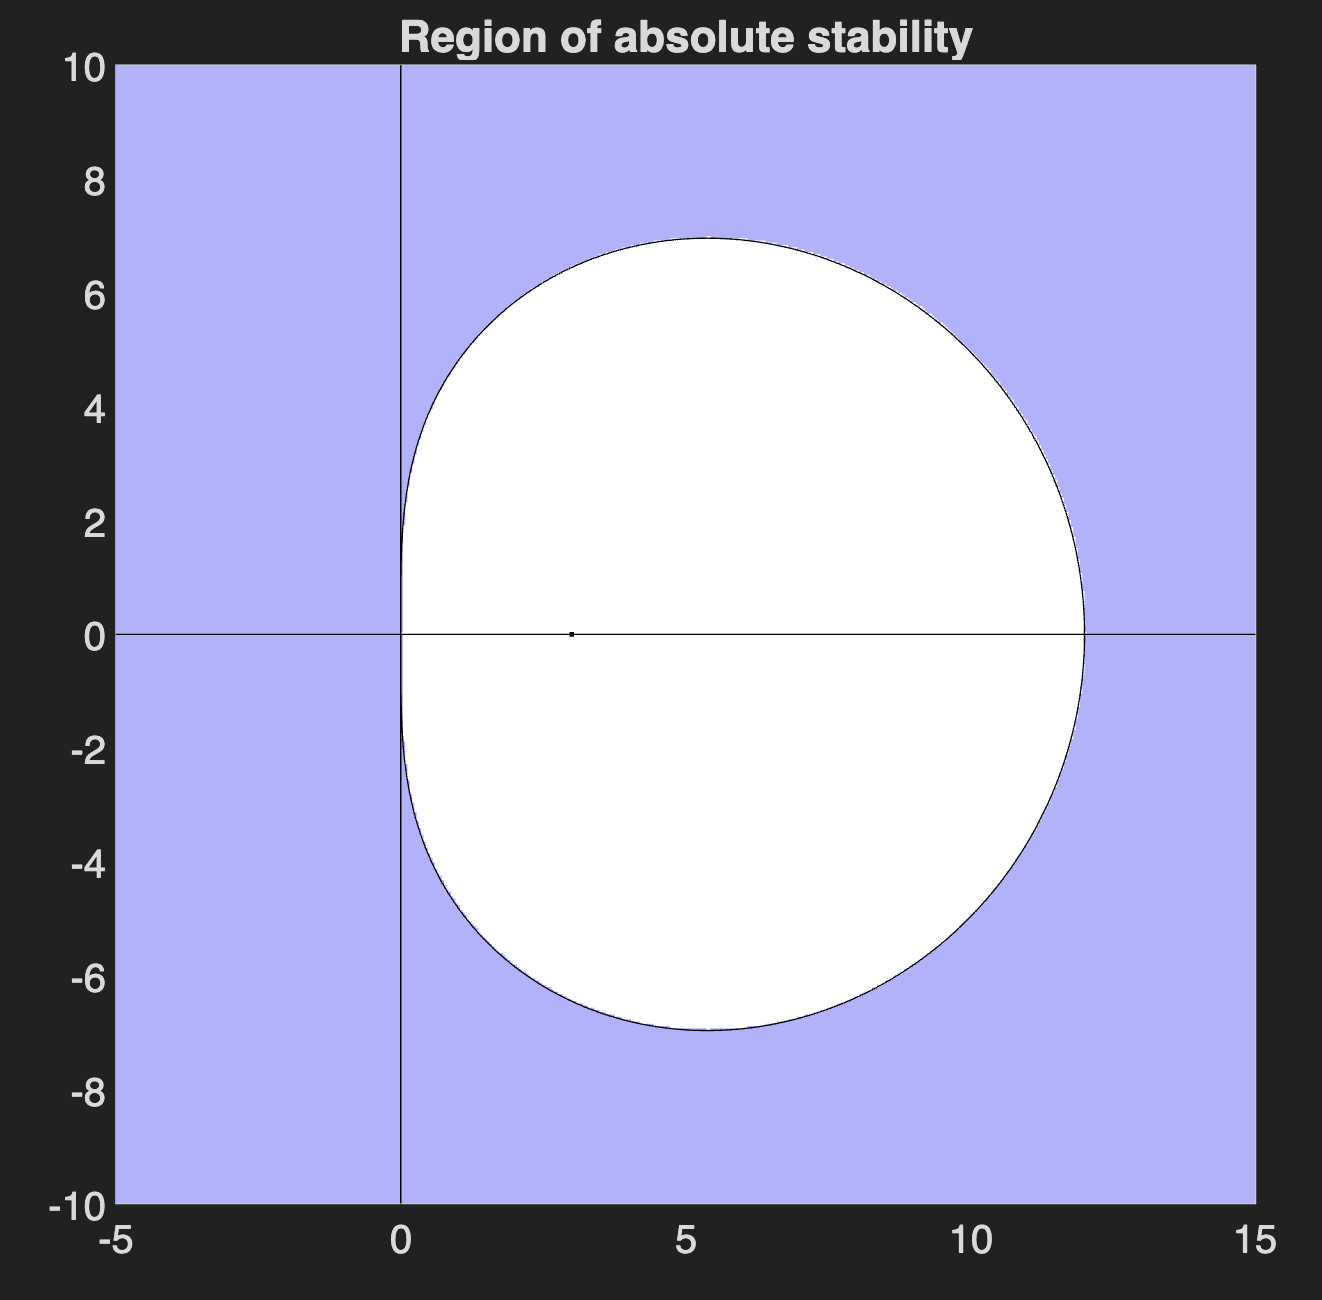
\includegraphics[scale=0.3]{Screenshot 2026-03-06 at 5.48.07 PM.png}
    \end{center}
\end{solution}

%%%%%%%%%%%%%%%%%%%%%%%%%%%%%%%%%%%%%%%%%%%%%%%%%%
%%%%%%%%%%%%%%%%%%%%%%%%%%%%%%%%%%%%%%%%%%%%%%%%%%
%%%%%%%%%%%%%%%%%%%%%%%%%%%%%%%%%%%%%%%%%%%%%%%%%%
\begin{exercise}[manual-num={8.4}]
\end{exercise}
\begin{solution}
Using the test problem $u' = \lambda u$, we have:
    \begin{equation*}
    \begin{split}
        U^\ast = U^n + \frac{z}{2}U^\ast.
    \end{split}
    \end{equation*}
Solving for $U^\ast$ gives:
    \begin{equation*}
    \begin{split}
        U^\ast = \frac{U^n}{1 - \frac{z}{2}}.
    \end{split}
    \end{equation*}
Hence:
    \begin{equation*}
    \begin{split}
        U^{n+1} 
        & = U^n + zU^\ast \\
        & = U^n + \frac{zU^n}{1- \frac{z}{2}} \\
        & = \left( 1 + \frac{z}{1 - \frac{z}{2}} \right)U^n.
    \end{split}
    \end{equation*}
The stability function is then given by $R(z) = (1 + \frac{z}{1 - \frac{z}{2}})$. Expressing $\frac{z}{1 - \frac{z}{2}}$ as its taylor series, we have:
    \begin{equation*}
    \begin{split}
        R(z) = 1 + z + \frac{z^2}{2} + \frac{z^3}{4} + \frac{z^4}{8}+...
    \end{split}
    \end{equation*}
Compared to the taylor expansion of $e^z$, note that $R(z)$ differs after the $z^2$ term. Hence the method is second order accurate.
\end{solution}
%%%%%%%%%%%%%%%%%%%%%%%%%%%%%%%%%%%%%%%%%%%%%%%%%%
%%%%%%%%%%%%%%%%%%%%%%%%%%%%%%%%%%%%%%%%%%%%%%%%%%
%%%%%%%%%%%%%%%%%%%%%%%%%%%%%%%%%%%%%%%%%%%%%%%%%%
\begin{exercise}[manual-num={9.1}]
    
\end{exercise}
\begin{solution}
    (a) Manipulating our original scheme and re-indexing, we get:
        \begin{equation*}
        \begin{split}
            \frac{U_i^{n+1} - U_i^{n-1}}{2k} = \frac{U_{i-1}^n - 2 U_n^n + U_{i+1}^n}{h^2}.
        \end{split}
        \end{equation*}
    Thus:
        \begin{equation*}
        \begin{split}
            \tau = \frac{u(x_1,t_{n+1}) - u(x_1,t_{n-1})}{2k} - \frac{u(x_{i-1},t_n) - 2u(x_1,t_n) + u(x_{i+1},t_n)}{h^2}.
        \end{split}
        \end{equation*}
    Taylor expanding yields:
        \begin{equation*}
        \begin{split}
            \frac{u(x_1,t_{n+1}) - u(x_1,t_{n-1})}{2k} = u_t + \frac{k^2}{6}u_{ttt} + O(k^4).
        \end{split}
        \end{equation*}
    Since $u_t = u_xx$, the right hand side becomes:
        \begin{equation*}
        \begin{split}
            \frac{u(x_1,t_{n+1}) - u(x_1,t_{n-1})}{2k} = u_xx + \frac{k^2}{6}u_{xxxx} + O(k^4).
        \end{split}
        \end{equation*}
    Hence:
        \begin{equation*}
        \begin{split}
            \tau = (u_t - u_{xx}) + \frac{k^2}{6}u_{ttt} - \frac{h^2}{12}u_{xxxx} + O(k^4) + O(h^2).
        \end{split}
        \end{equation*}
    Thus the order of accuracy is $O(k^2)$ and $O(h^2)$.

    (b) The eigenvalues satisfy $\frac{-4}{h^2} < \lambda_p < 0$. From the leapfrog scheme, we have: $$U^{n+2} = U^n + 2k\lambda U^{n+1}.$$ Taking $r = \lambda k$, the scheme can be rewritten as $z^2 -2rz - 1 = 0$. The roots of this polynomial are $z = r \pm \sqrt{r^2 + 1}$. Note that the modulus of $z$ is strictly greater than one, hence it is not stable.  
\end{solution}
    
%%%%%%%%%%%%%%%%%%%%%%%%%%%%%%%%%%%%%%%%%%%%%%%%%%
%%%%%%%%%%%%%%%%%%%%%%%%%%%%%%%%%%%%%%%%%%%%%%%%%%
%%%%%%%%%%%%%%%%%%%%%%%%%%%%%%%%%%%%%%%%%%%%%%%%%%
\begin{exercise}[manual-num={9.2}]
\end{exercise}
\begin{solution}
(a) After adjusting \texttt{heat\_CN.m} the following code outputs an error table and $\log$-$\log$ plot using \texttt{error\_table.m} and \texttt{error\_loglog.m}.

\begin{lstlisting}[style=editor]
mvals = [10 20 40 80 160];      
ntest = length(mvals);

hvals = zeros(ntest,1);
E     = zeros(ntest,1);

for j = 1:ntest
    [hvals(j),~,E(j)] = heat_CN(mvals(j)); 
end

error_table(hvals, E);
error_loglog(hvals, E);
\end{lstlisting}
\begin{lstlisting}[style=console]
>> hw6
 
WARNING *** k does not divide tfinal, k = 3.63636e-01
 
at time t = 1.09091e+00  max error =  2.52504e-03
 
WARNING *** k does not divide tfinal, k = 1.90476e-01
 
at time t = 9.52381e-01  max error =  9.07877e-04
 
WARNING *** k does not divide tfinal, k = 9.75610e-02
 
at time t = 9.75610e-01  max error =  1.53948e-04
 
WARNING *** k does not divide tfinal, k = 4.93827e-02
 
at time t = 9.87654e-01  max error =  3.89510e-05
 
WARNING *** k does not divide tfinal, k = 2.48447e-02
 
at time t = 9.93789e-01  max error =  9.80754e-06
 
      h        error       ratio       observed order
   0.09091   2.52504e-03       NaN             NaN
   0.04762   9.07877e-04   2.78125         1.58190
   0.02439   1.53948e-04   5.89730         2.65226
   0.01235   3.89510e-05   3.95235         2.01844
   0.00621   9.80754e-06   3.97154         2.00763
 
 
Least squares fit gives E(h) = 0.457212 * h^2.12203
 
>> 
\end{lstlisting}
\begin{center}
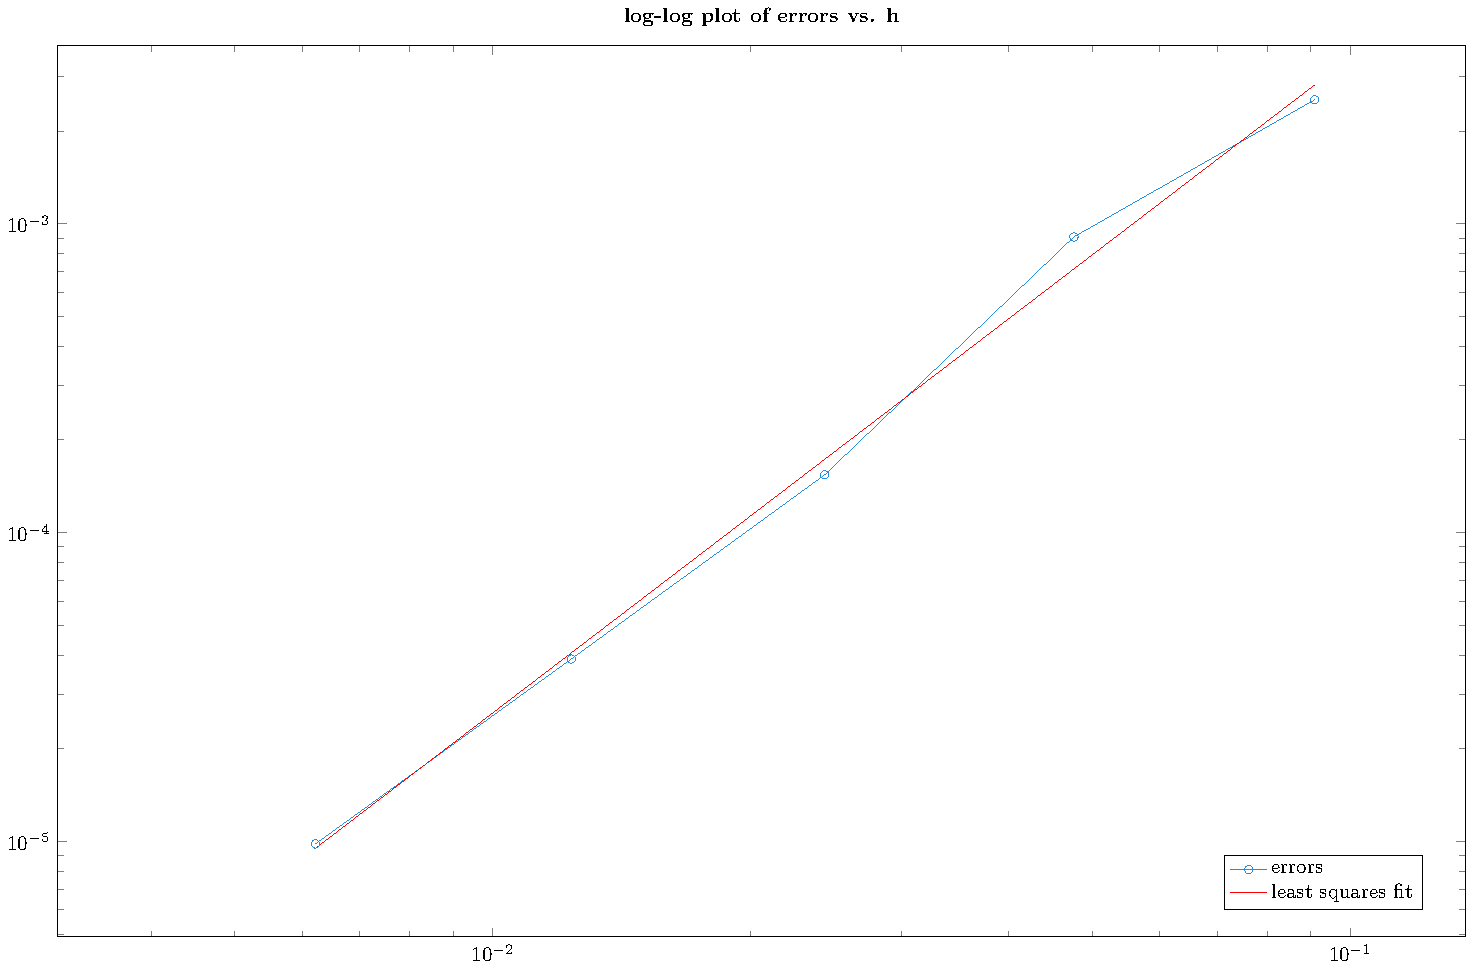
\includegraphics[scale=0.45]{p-9loglogplot.pdf}
\end{center}

(b) Below is the updated code using the Backward Euler method:
\begin{lstlisting}[style=editor]
function [h,k,error] = heat_CN1(m)

clf              % clear graphics
hold on          % Put all plots on the same graph (comment out if desired)

ax = 0;
bx = 1;
kappa = .02;               % heat conduction coefficient:
tfinal = 1;                % final time

h = (bx-ax)/(m+1);         % h = delta x
x = linspace(ax,bx,m+2)';  % note x(1)=0 and x(m+2)=1
                           % u(1)=g0 and u(m+2)=g1 are known from BC's
k = 24*h^2;                  % time step

nsteps = round(tfinal / k);    % number of time steps
%nplot = 1;      % plot solution every nplot time steps
                 % (set nplot=2 to plot every 2 time steps, etc.)
nplot = nsteps;  % only plot at final time

if abs(k*nsteps - tfinal) > 1e-5
   % The last step won't go exactly to tfinal.
   disp(' ')
   disp(sprintf('WARNING *** k does not divide tfinal, k = %9.5e',k))
   disp(' ')
   end


% true solution for comparison:
% For Gaussian initial conditions u(x,0) = exp(-beta * (x-0.4)^2)
beta = 150;
utrue = @(x,t) exp(-(x-0.4).^2 / (4*kappa*t + 1/beta)) / sqrt(4*beta*kappa*t+1);

% initial conditions:
u0 = utrue(x,0);


% Each time step we solve MOL system U' = AU + g using the Trapezoidal method

% set up matrices:
r = kappa* k/(h^2);
e = ones(m,1);
A = spdiags([e -2*e e], [-1 0 1], m, m);
%A1 = eye(m) - r * A;
A2 = eye(m) + r * A;


% initial data on fine grid for plotting:
xfine = linspace(ax,bx,1001);
ufine = utrue(xfine,0);

% initialize u and plot:
tn = 0;
u = u0;

plot(x,u,'b.-', xfine,ufine,'r')
legend('computed','true')
title('Initial data at time = 0')

input('Hit <return> to continue  ');


% main time-stepping loop:

for n = 1:nsteps
     tnp = tn + k;   % = t_{n+1}

     % boundary values u(0,t) and u(1,t) at times tn and tnp:

     g0n = u(1);
     g1n = u(m+2);
     g0np = utrue(ax,tnp);
     g1np = utrue(bx,tnp);

     % compute right hand side for linear system:
     uint = u(2:(m+1));   % interior points (unknowns)
     rhs = A2*uint;
     % fix-up right hand side using BC's (i.e. add vector g to A2*uint)
     rhs(1) = rhs(1) + r*(g0n);
     rhs(m) = rhs(m) + r*(g1n);

     % solve linear system:
     uint = rhs;

     % augment with boundary values:
     u = [g0np; uint; g1np];

     % plot results at desired times:
     if mod(n,nplot)==0 | n==nsteps
        ufine = utrue(xfine,tnp);
        plot(x,u,'b.-', xfine,ufine,'r')
        title(sprintf('t = %9.5e  after %4i time steps with %5i grid points',...
                       tnp,n,m+2))
        error = max(abs(u-utrue(x,tnp)));
        disp(sprintf('at time t = %9.5e  max error =  %9.5e',tnp,error))
        if n<nsteps, input('Hit <return> to continue  '); end;
        end

     tn = tnp;   % for next time step
     end   
\end{lstlisting}
Using the same error-analysis in part (a), we get the following output:
\begin{lstlisting}[style=console]
>> hw6partb
 
WARNING *** k does not divide tfinal, k = 1.98347e-01
 
Hit <return> to continue  
at time t = 9.91736e-01  max error =  3.04307e-02
 
WARNING *** k does not divide tfinal, k = 5.44218e-02
 
Hit <return> to continue  
at time t = 9.79592e-01  max error =  3.09354e-03
 
WARNING *** k does not divide tfinal, k = 1.42772e-02
 
Hit <return> to continue  
at time t = 9.99405e-01  max error =  8.14505e-04
 
WARNING *** k does not divide tfinal, k = 3.65798e-03
 
Hit <return> to continue  

at time t = 9.98628e-01  max error =  2.09904e-04
 
WARNING *** k does not divide tfinal, k = 9.25890e-04
 
Hit <return> to continue  
at time t = 9.99961e-01  max error =  5.31161e-05
 
WARNING *** k does not divide tfinal, k = 2.32917e-04
 
Hit <return> to continue  
at time t = 9.99913e-01  max error =  1.33685e-05
 
      h        error       ratio       observed order
   0.09091   3.04307e-02       NaN             NaN
   0.04762   3.09354e-03   9.83683         3.53547
   0.02439   8.14505e-04   3.79807         1.99461
   0.01235   2.09904e-04   3.88037         1.99145
   0.00621   5.31161e-05   3.95179         2.00038
   0.00312   1.33685e-05   3.97324         1.99929
 
 
Least squares fit gives E(h) = 3.70715 * h^2.20379
 
>>    
\end{lstlisting}
Hence the method is $O(h^2)$ accurate.

(c) I was not getting an unstable output. Unsure of what I did wrong.

\end{solution}

%%%%%%%%%%%%%%%%%%%%%%%%%%%%%%%%%%%%%%%%%%%%%%%%%%
%%%%%%%%%%%%%%%%%%%%%%%%%%%%%%%%%%%%%%%%%%%%%%%%%%
%%%%%%%%%%%%%%%%%%%%%%%%%%%%%%%%%%%%%%%%%%%%%%%%%%
\begin{exercise}[manual-num={9.3}]
\end{exercise}
\begin{solution}
Below is the updated code.


\begin{lstlisting}[style=editor]
function [h,k,error] = heat_CN(m)

clf              % clear graphics
hold on          % Put all plots on the same graph (comment out if desired)

ax = -1;
bx = 1;
kappa = .02;               % heat conduction coefficient:
tfinal = 1;                % final time

h = (bx-ax)/(m+1);         % h = delta x
x = linspace(ax,bx,m+2)';  % note x(1)=0 and x(m+2)=1
                           % u(1)=g0 and u(m+2)=g1 are known from BC's
k = 4*h;                   % time step

nsteps = round(tfinal / k);    % number of time steps
%nplot = 1;      % plot solution every nplot time steps
                 % (set nplot=2 to plot every 2 time steps, etc.)
nplot = nsteps;  % only plot at final time

if abs(k*nsteps - tfinal) > 1e-5
   % The last step won't go exactly to tfinal.
   disp(' ')
   disp(sprintf('WARNING *** k does not divide tfinal, k = %9.5e',k))
   disp(' ')
   end


% true solution for comparison:
utrue = @(x,t) 0.5 * erfc( x ./ sqrt(4*kappa*t) );

% initial conditions (consistent with utrue as t -> 0+):
u0 = double(x < 0);   % 1 if x<0, 0 if x>=0


% Each time step we solve MOL system U' = AU + g using the Trapezoidal method

% set up matrices:
r = (1/2) * kappa* k/(h^2);
e = ones(m,1);
A = spdiags([e -2*e e], [-1 0 1], m, m);
A1 = eye(m) - r * A;
A2 = eye(m) + r * A;


% initial data on fine grid for plotting:
xfine = linspace(ax,bx,1001);
ufine = utrue(xfine,0);

% initialize u and plot:
tn = 0;
u = u0;

plot(x,u,'b.-', xfine,ufine,'r')
legend('computed','true')
title('Initial data at time = 0')

input('Hit <return> to continue  ');


% main time-stepping loop:

for n = 1:nsteps
     tnp = tn + k;   % = t_{n+1}

     % boundary values u(0,t) and u(1,t) at times tn and tnp:

     g0n = u(1);
     g1n = u(m+2);
     g0np = utrue(ax,tnp);
     g1np = utrue(bx,tnp);

     % compute right hand side for linear system:
     uint = u(2:(m+1));   % interior points (unknowns)
     rhs = A2*uint;
     % fix-up right hand side using BC's (i.e. add vector g to A2*uint)
     rhs(1) = rhs(1) + r*(g0n + g0np);
     rhs(m) = rhs(m) + r*(g1n + g1np);

     % solve linear system:
     uint = A1\rhs;

     % augment with boundary values:
     u = [g0np; uint; g1np];

     % plot results at desired times:
     if mod(n,nplot)==0 | n==nsteps
        ufine = utrue(xfine,tnp);
        plot(x,u,'b.-', xfine,ufine,'r')
        title(sprintf('t = %9.5e  after %4i time steps with %5i grid points',...
                       tnp,n,m+2))
        error = max(abs(u-utrue(x,tnp)));
        disp(sprintf('at time t = %9.5e  max error =  %9.5e',tnp,error))
        if n<nsteps, input('Hit <return> to continue  '); end;
        end

     tn = tnp;   % for next time step
     end
\end{lstlisting}

(a) Attached is the output when $m = 39$ and $k = 4h$.
    \begin{center}
    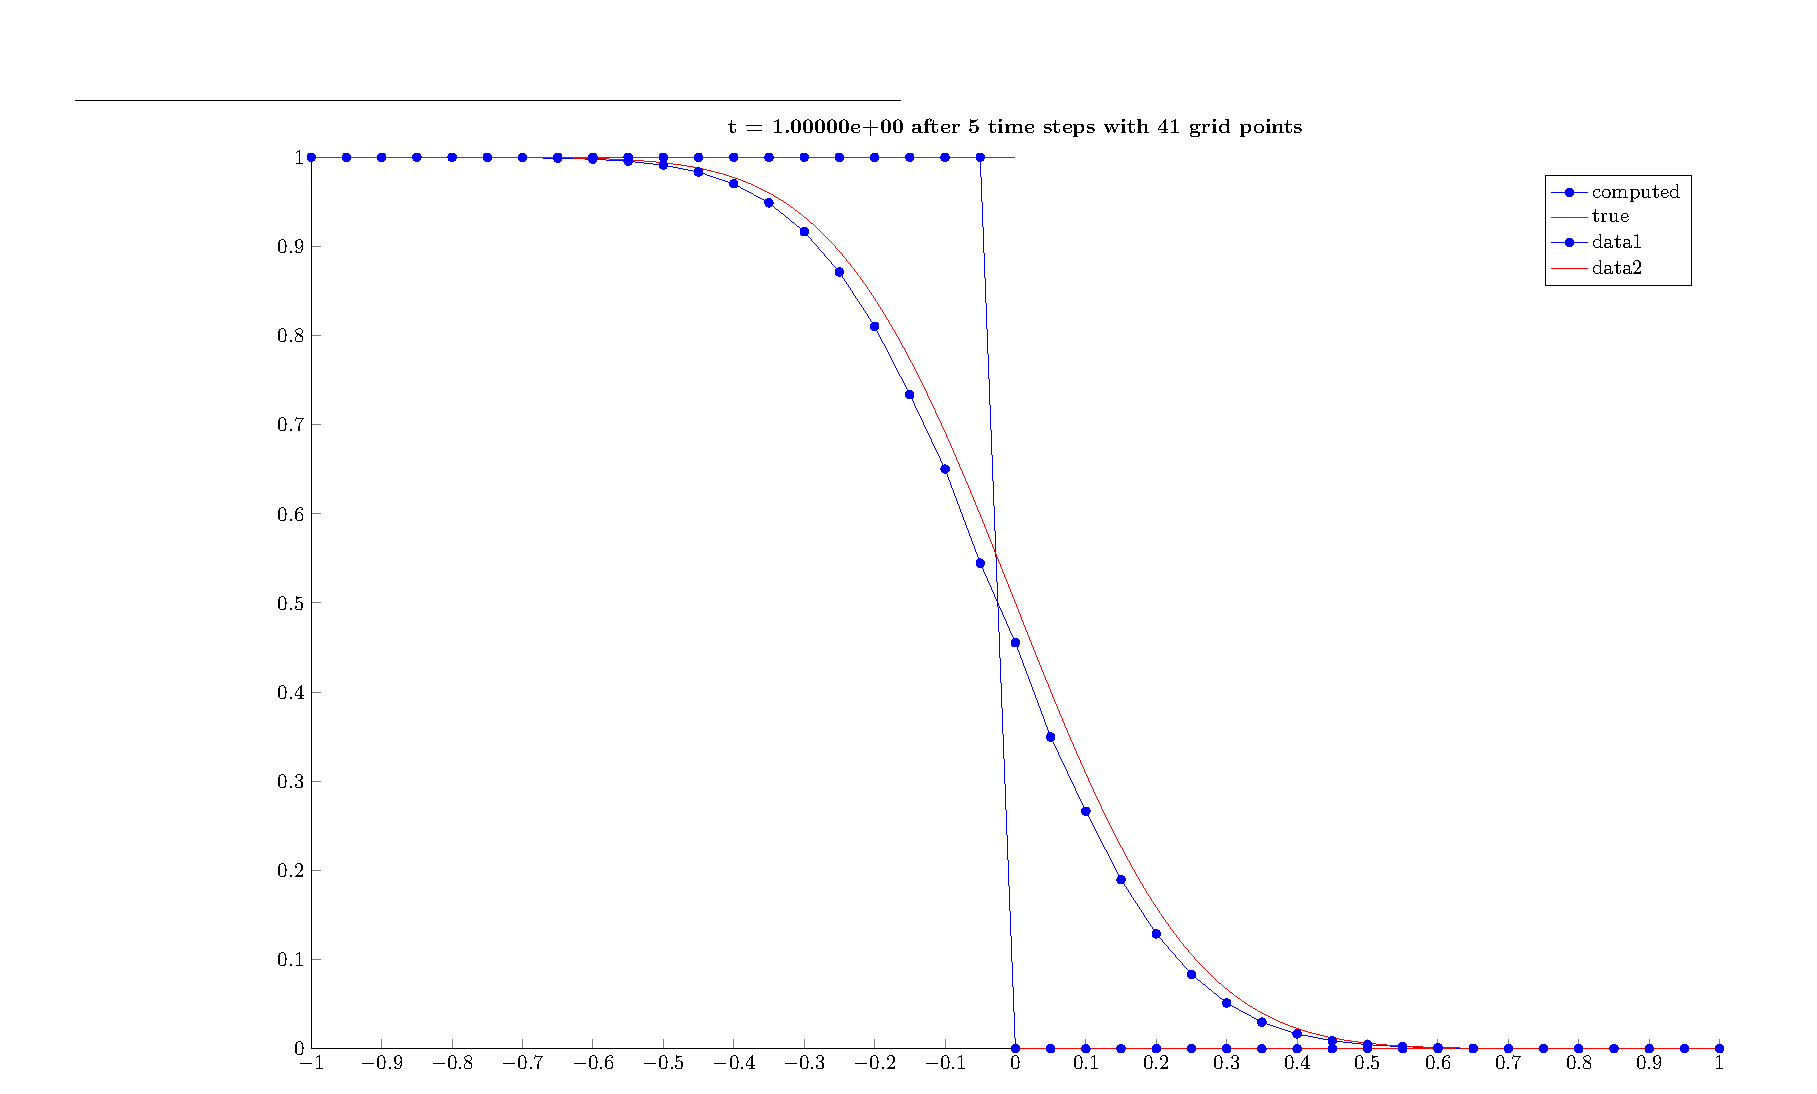
\includegraphics[scale=.45]{heatoutput39.pdf}
    \end{center}

(b) Attached is the output when $m = 38$ and $k = 4h$.
    \begin{center}
    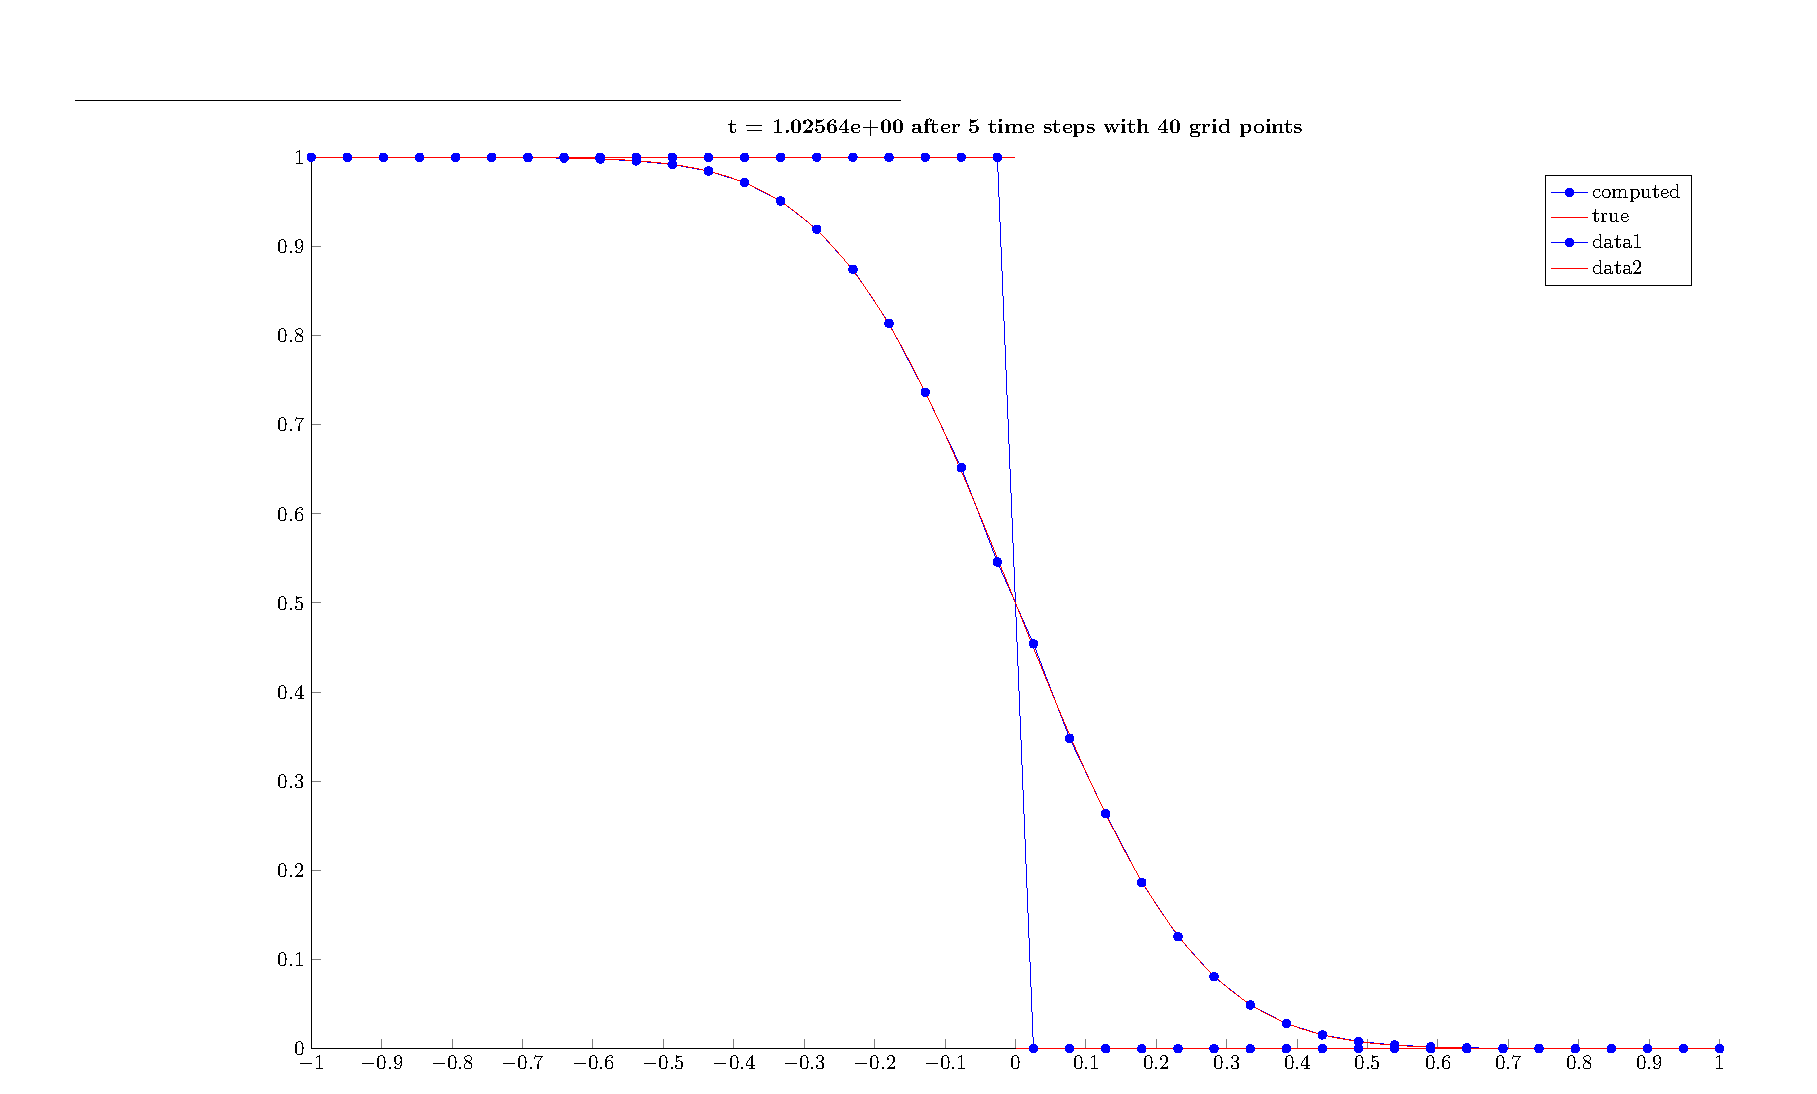
\includegraphics[scale=.45]{heatoutput38.pdf}
    \end{center}
    The better results for $m =38$ are due to $x=0$ lying between two grid points. The order of accuracy is first-order as the solution is not smooth at $t=0$, reducing the usual second-order behavior of Crank-Nicolson method.
\end{solution}
%%%%%%%%%%%%%%%%%%%%%%%%%%%%%%%%%%%%%%%%%%%%%%%%%%
%%%%%%%%%%%%%%%%%%%%%%%%%%%%%%%%%%%%%%%%%%%%%%%%%%
%%%%%%%%%%%%%%%%%%%%%%%%%%%%%%%%%%%%%%%%%%%%%%%%%%


\end{document}